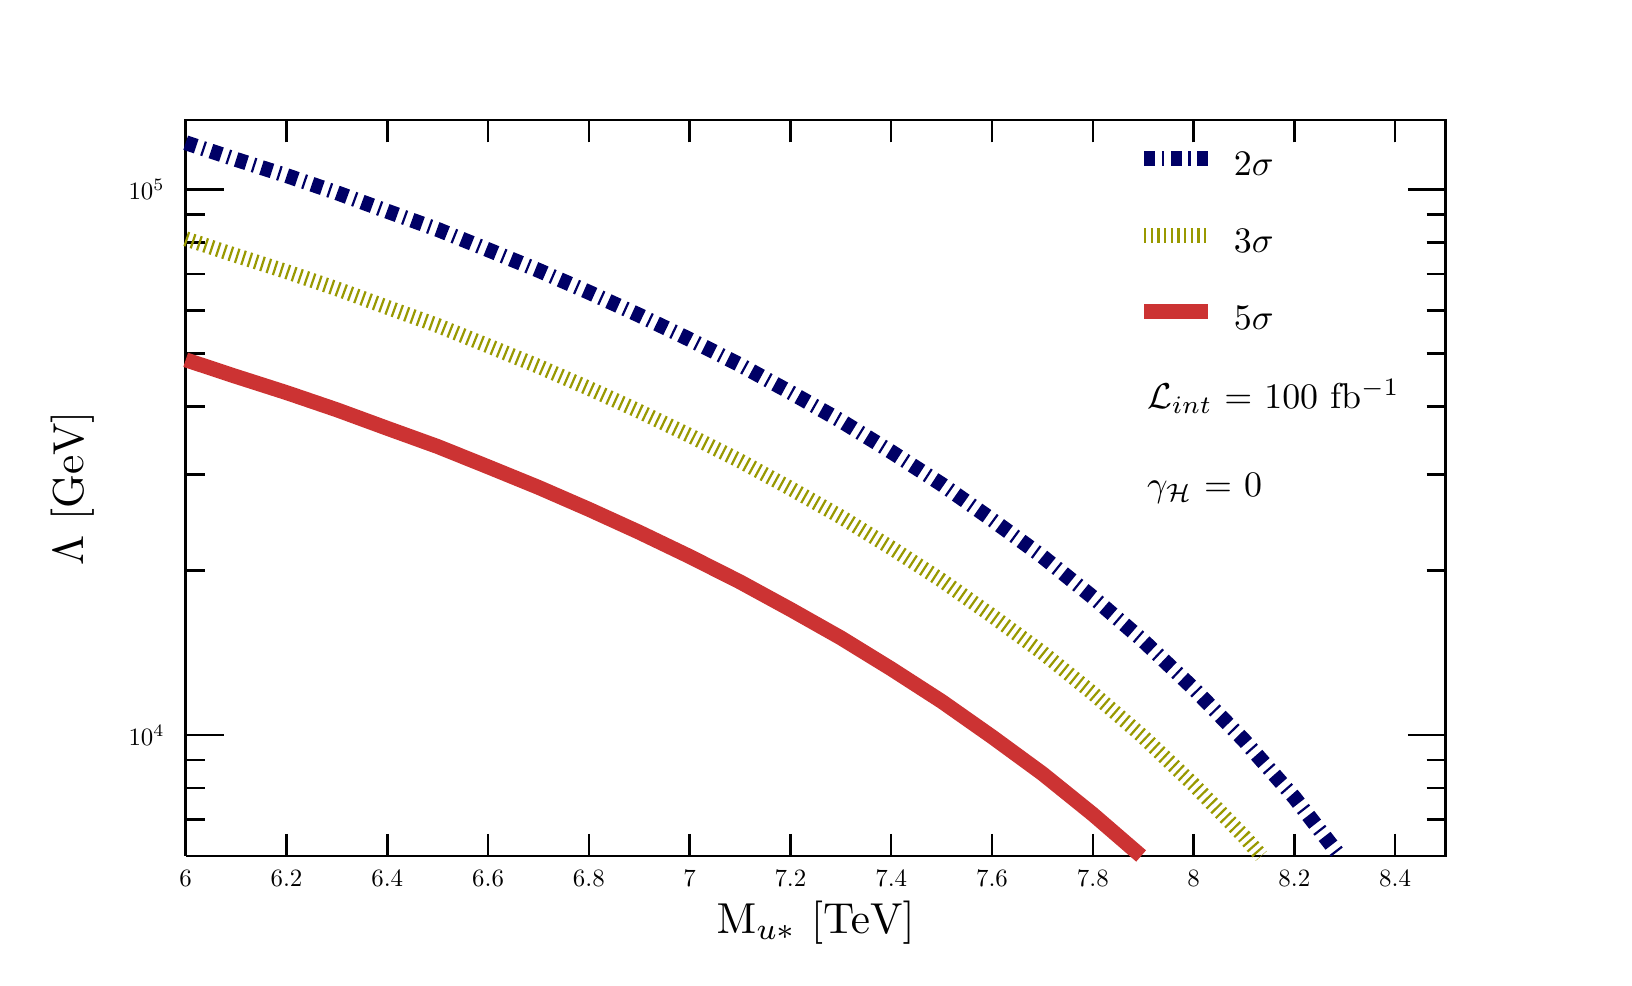
\begin{tikzpicture}
\pgfdeclareplotmark{cross} {
\pgfpathmoveto{\pgfpoint{-0.3\pgfplotmarksize}{\pgfplotmarksize}}
\pgfpathlineto{\pgfpoint{+0.3\pgfplotmarksize}{\pgfplotmarksize}}
\pgfpathlineto{\pgfpoint{+0.3\pgfplotmarksize}{0.3\pgfplotmarksize}}
\pgfpathlineto{\pgfpoint{+1\pgfplotmarksize}{0.3\pgfplotmarksize}}
\pgfpathlineto{\pgfpoint{+1\pgfplotmarksize}{-0.3\pgfplotmarksize}}
\pgfpathlineto{\pgfpoint{+0.3\pgfplotmarksize}{-0.3\pgfplotmarksize}}
\pgfpathlineto{\pgfpoint{+0.3\pgfplotmarksize}{-1.\pgfplotmarksize}}
\pgfpathlineto{\pgfpoint{-0.3\pgfplotmarksize}{-1.\pgfplotmarksize}}
\pgfpathlineto{\pgfpoint{-0.3\pgfplotmarksize}{-0.3\pgfplotmarksize}}
\pgfpathlineto{\pgfpoint{-1.\pgfplotmarksize}{-0.3\pgfplotmarksize}}
\pgfpathlineto{\pgfpoint{-1.\pgfplotmarksize}{0.3\pgfplotmarksize}}
\pgfpathlineto{\pgfpoint{-0.3\pgfplotmarksize}{0.3\pgfplotmarksize}}
\pgfpathclose
\pgfusepathqstroke
}
\pgfdeclareplotmark{cross*} {
\pgfpathmoveto{\pgfpoint{-0.3\pgfplotmarksize}{\pgfplotmarksize}}
\pgfpathlineto{\pgfpoint{+0.3\pgfplotmarksize}{\pgfplotmarksize}}
\pgfpathlineto{\pgfpoint{+0.3\pgfplotmarksize}{0.3\pgfplotmarksize}}
\pgfpathlineto{\pgfpoint{+1\pgfplotmarksize}{0.3\pgfplotmarksize}}
\pgfpathlineto{\pgfpoint{+1\pgfplotmarksize}{-0.3\pgfplotmarksize}}
\pgfpathlineto{\pgfpoint{+0.3\pgfplotmarksize}{-0.3\pgfplotmarksize}}
\pgfpathlineto{\pgfpoint{+0.3\pgfplotmarksize}{-1.\pgfplotmarksize}}
\pgfpathlineto{\pgfpoint{-0.3\pgfplotmarksize}{-1.\pgfplotmarksize}}
\pgfpathlineto{\pgfpoint{-0.3\pgfplotmarksize}{-0.3\pgfplotmarksize}}
\pgfpathlineto{\pgfpoint{-1.\pgfplotmarksize}{-0.3\pgfplotmarksize}}
\pgfpathlineto{\pgfpoint{-1.\pgfplotmarksize}{0.3\pgfplotmarksize}}
\pgfpathlineto{\pgfpoint{-0.3\pgfplotmarksize}{0.3\pgfplotmarksize}}
\pgfpathclose
\pgfusepathqfillstroke
}
\pgfdeclareplotmark{newstar} {
\pgfpathmoveto{\pgfqpoint{0pt}{\pgfplotmarksize}}
\pgfpathlineto{\pgfqpointpolar{44}{0.5\pgfplotmarksize}}
\pgfpathlineto{\pgfqpointpolar{18}{\pgfplotmarksize}}
\pgfpathlineto{\pgfqpointpolar{-20}{0.5\pgfplotmarksize}}
\pgfpathlineto{\pgfqpointpolar{-54}{\pgfplotmarksize}}
\pgfpathlineto{\pgfqpointpolar{-90}{0.5\pgfplotmarksize}}
\pgfpathlineto{\pgfqpointpolar{234}{\pgfplotmarksize}}
\pgfpathlineto{\pgfqpointpolar{198}{0.5\pgfplotmarksize}}
\pgfpathlineto{\pgfqpointpolar{162}{\pgfplotmarksize}}
\pgfpathlineto{\pgfqpointpolar{134}{0.5\pgfplotmarksize}}
\pgfpathclose
\pgfusepathqstroke
}
\pgfdeclareplotmark{newstar*} {
\pgfpathmoveto{\pgfqpoint{0pt}{\pgfplotmarksize}}
\pgfpathlineto{\pgfqpointpolar{44}{0.5\pgfplotmarksize}}
\pgfpathlineto{\pgfqpointpolar{18}{\pgfplotmarksize}}
\pgfpathlineto{\pgfqpointpolar{-20}{0.5\pgfplotmarksize}}
\pgfpathlineto{\pgfqpointpolar{-54}{\pgfplotmarksize}}
\pgfpathlineto{\pgfqpointpolar{-90}{0.5\pgfplotmarksize}}
\pgfpathlineto{\pgfqpointpolar{234}{\pgfplotmarksize}}
\pgfpathlineto{\pgfqpointpolar{198}{0.5\pgfplotmarksize}}
\pgfpathlineto{\pgfqpointpolar{162}{\pgfplotmarksize}}
\pgfpathlineto{\pgfqpointpolar{134}{0.5\pgfplotmarksize}}
\pgfpathclose
\pgfusepathqfillstroke
}
\definecolor{c}{rgb}{1,1,1};
\draw [color=c, fill=c] (0,0) rectangle (20,11.6806);
\draw [color=c, fill=c] (2,1.16806) rectangle (18,10.5125);
\definecolor{c}{rgb}{0,0,0};
\draw [c,line width=0.9] (2,1.16806) -- (2,10.5125) -- (18,10.5125) -- (18,1.16806) -- (2,1.16806);
\definecolor{c}{rgb}{1,1,1};
\draw [color=c, fill=c] (2,1.16806) rectangle (18,10.5125);
\definecolor{c}{rgb}{0,0,0};
\draw [c,line width=0.9] (2,1.16806) -- (2,10.5125) -- (18,10.5125) -- (18,1.16806) -- (2,1.16806);
\draw [c,line width=0.9] (2,1.16806) -- (18,1.16806);
\draw (10,0.327056) node[scale=1.56475, color=c, rotate=0]{M$_{u*}$ [TeV]};
\draw [c,line width=0.9] (2,1.44839) -- (2,1.16806);
\draw [c,line width=0.9] (3.28,1.44839) -- (3.28,1.16806);
\draw [c,line width=0.9] (4.56,1.44839) -- (4.56,1.16806);
\draw [c,line width=0.9] (5.84,1.44839) -- (5.84,1.16806);
\draw [c,line width=0.9] (7.12,1.44839) -- (7.12,1.16806);
\draw [c,line width=0.9] (8.4,1.44839) -- (8.4,1.16806);
\draw [c,line width=0.9] (9.68,1.44839) -- (9.68,1.16806);
\draw [c,line width=0.9] (10.96,1.44839) -- (10.96,1.16806);
\draw [c,line width=0.9] (12.24,1.44839) -- (12.24,1.16806);
\draw [c,line width=0.9] (13.52,1.44839) -- (13.52,1.16806);
\draw [c,line width=0.9] (14.8,1.44839) -- (14.8,1.16806);
\draw [c,line width=0.9] (16.08,1.44839) -- (16.08,1.16806);
\draw [c,line width=0.9] (17.36,1.44839) -- (17.36,1.16806);
\draw [c,line width=0.9] (17.36,1.44839) -- (17.36,1.16806);
\draw [anchor=base] (2,0.782598) node[scale=0.900036, color=c, rotate=0]{6};
\draw [anchor=base] (3.28,0.782598) node[scale=0.900036, color=c, rotate=0]{6.2};
\draw [anchor=base] (4.56,0.782598) node[scale=0.900036, color=c, rotate=0]{6.4};
\draw [anchor=base] (5.84,0.782598) node[scale=0.900036, color=c, rotate=0]{6.6};
\draw [anchor=base] (7.12,0.782598) node[scale=0.900036, color=c, rotate=0]{6.8};
\draw [anchor=base] (8.4,0.782598) node[scale=0.900036, color=c, rotate=0]{7};
\draw [anchor=base] (9.68,0.782598) node[scale=0.900036, color=c, rotate=0]{7.2};
\draw [anchor=base] (10.96,0.782598) node[scale=0.900036, color=c, rotate=0]{7.4};
\draw [anchor=base] (12.24,0.782598) node[scale=0.900036, color=c, rotate=0]{7.6};
\draw [anchor=base] (13.52,0.782598) node[scale=0.900036, color=c, rotate=0]{7.8};
\draw [anchor=base] (14.8,0.782598) node[scale=0.900036, color=c, rotate=0]{8};
\draw [anchor=base] (16.08,0.782598) node[scale=0.900036, color=c, rotate=0]{8.2};
\draw [anchor=base] (17.36,0.782598) node[scale=0.900036, color=c, rotate=0]{8.4};
\draw [c,line width=0.9] (2,10.5125) -- (18,10.5125);
\draw [c,line width=0.9] (2,10.2322) -- (2,10.5125);
\draw [c,line width=0.9] (3.28,10.2322) -- (3.28,10.5125);
\draw [c,line width=0.9] (4.56,10.2322) -- (4.56,10.5125);
\draw [c,line width=0.9] (5.84,10.2322) -- (5.84,10.5125);
\draw [c,line width=0.9] (7.12,10.2322) -- (7.12,10.5125);
\draw [c,line width=0.9] (8.4,10.2322) -- (8.4,10.5125);
\draw [c,line width=0.9] (9.68,10.2322) -- (9.68,10.5125);
\draw [c,line width=0.9] (10.96,10.2322) -- (10.96,10.5125);
\draw [c,line width=0.9] (12.24,10.2322) -- (12.24,10.5125);
\draw [c,line width=0.9] (13.52,10.2322) -- (13.52,10.5125);
\draw [c,line width=0.9] (14.8,10.2322) -- (14.8,10.5125);
\draw [c,line width=0.9] (16.08,10.2322) -- (16.08,10.5125);
\draw [c,line width=0.9] (17.36,10.2322) -- (17.36,10.5125);
\draw [c,line width=0.9] (17.36,10.2322) -- (17.36,10.5125);
\draw [c,line width=0.9] (2,1.16806) -- (2,10.5125);
\draw (0.56,5.84029) node[scale=1.56475, color=c, rotate=90]{$\Lambda$ [GeV]};
\draw [c,line width=0.9] (2.24,1.16855) -- (2,1.16855);
\draw [c,line width=0.9] (2.24,1.6323) -- (2,1.6323);
\draw [c,line width=0.9] (2.24,2.03402) -- (2,2.03402);
\draw [c,line width=0.9] (2.24,2.38837) -- (2,2.38837);
\draw [c,line width=0.9] (2.48,2.70534) -- (2,2.70534);
\draw [anchor= east] (1.844,2.70534) node[scale=0.900036, color=c, rotate=0]{$10^{4}$};
\draw [c,line width=0.9] (2.24,4.79062) -- (2,4.79062);
\draw [c,line width=0.9] (2.24,6.01044) -- (2,6.01044);
\draw [c,line width=0.9] (2.24,6.87591) -- (2,6.87591);
\draw [c,line width=0.9] (2.24,7.54722) -- (2,7.54722);
\draw [c,line width=0.9] (2.24,8.09573) -- (2,8.09573);
\draw [c,line width=0.9] (2.24,8.55948) -- (2,8.55948);
\draw [c,line width=0.9] (2.24,8.9612) -- (2,8.9612);
\draw [c,line width=0.9] (2.24,9.31554) -- (2,9.31554);
\draw [c,line width=0.9] (2.48,9.63251) -- (2,9.63251);
\draw [anchor= east] (1.844,9.63251) node[scale=0.900036, color=c, rotate=0]{$10^{5}$};
\draw [c,line width=0.9] (18,1.16806) -- (18,10.5125);
\draw [c,line width=0.9] (17.76,1.16855) -- (18,1.16855);
\draw [c,line width=0.9] (17.76,1.6323) -- (18,1.6323);
\draw [c,line width=0.9] (17.76,2.03402) -- (18,2.03402);
\draw [c,line width=0.9] (17.76,2.38837) -- (18,2.38837);
\draw [c,line width=0.9] (17.52,2.70534) -- (18,2.70534);
\draw [c,line width=0.9] (17.76,4.79062) -- (18,4.79062);
\draw [c,line width=0.9] (17.76,6.01044) -- (18,6.01044);
\draw [c,line width=0.9] (17.76,6.87591) -- (18,6.87591);
\draw [c,line width=0.9] (17.76,7.54722) -- (18,7.54722);
\draw [c,line width=0.9] (17.76,8.09573) -- (18,8.09573);
\draw [c,line width=0.9] (17.76,8.55948) -- (18,8.55948);
\draw [c,line width=0.9] (17.76,8.9612) -- (18,8.9612);
\draw [c,line width=0.9] (17.76,9.31554) -- (18,9.31554);
\draw [c,line width=0.9] (17.52,9.63251) -- (18,9.63251);
\definecolor{c}{rgb}{0,0,0.4};
\draw [c,dash pattern=on 4.00pt off 2.40pt on 0.80pt off 2.40pt ,line width=5.4] (2,10.226) -- (2.64,10.0141) -- (3.28,9.80923) -- (3.92,9.59105) -- (4.56,9.35602) -- (5.2,9.12479) -- (5.84,8.86737) -- (6.48,8.60608) -- (7.12,8.32731) --
 (7.76,8.03572) -- (8.4,7.72815) -- (9.04,7.40521) -- (9.68,7.05635) -- (10.32,6.69499) -- (10.96,6.30128) -- (11.6,5.88878) -- (12.24,5.43916) -- (12.88,4.97103) -- (13.52,4.45476) -- (14.16,3.90176) -- (14.8,3.29466) -- (15.44,2.63751) --
 (16.08,1.9103) -- (16.6578,1.16806);
\definecolor{c}{rgb}{0.6,0.6,0};
\draw [c,dash pattern=on 0.80pt off 1.60pt ,line width=5.4] (2,9.00613) -- (2.64,8.79429) -- (3.28,8.58941) -- (3.92,8.37124) -- (4.56,8.13621) -- (5.2,7.90498) -- (5.84,7.64755) -- (6.48,7.38626) -- (7.12,7.1075) -- (7.76,6.81591) -- (8.4,6.50834)
 -- (9.04,6.1854) -- (9.68,5.83653) -- (10.32,5.47517) -- (10.96,5.08146) -- (11.6,4.66898) -- (12.24,4.21934) -- (12.88,3.75121) -- (13.52,3.23493) -- (14.16,2.68194) -- (14.8,2.07484) -- (15.44,1.4177) -- (15.6597,1.16806);
\definecolor{c}{rgb}{0.8,0.2,0.2};
\draw [c,line width=5.4] (2,7.46935) -- (2.64,7.25751) -- (3.28,7.05262) -- (3.92,6.83445) -- (4.56,6.59943) -- (5.2,6.3682) -- (5.84,6.11077) -- (6.48,5.84947) -- (7.12,5.57071) -- (7.76,5.27913) -- (8.4,4.97156) -- (9.04,4.64861) -- (9.68,4.29975)
 -- (10.32,3.93839) -- (10.96,3.54468) -- (11.6,3.13218) -- (12.24,2.68256) -- (12.88,2.21443) -- (13.52,1.69816) -- (14.1335,1.16806);
\definecolor{c}{rgb}{0,0,0};
\draw (10,11.301) node[scale=1.2177, color=c, rotate=0]{ };
\draw [anchor=base west] (15.15,9.80681) node[scale=1.29711, color=c, rotate=0]{$2\sigma$};
\definecolor{c}{rgb}{0,0,0.4};
\draw [c,dash pattern=on 4.00pt off 2.40pt on 0.80pt off 2.40pt ,line width=5.4] (14.1725,10.0258) -- (14.9775,10.0258);
\definecolor{c}{rgb}{0,0,0};
\draw [anchor=base west] (15.15,8.83343) node[scale=1.29711, color=c, rotate=0]{$3\sigma$};
\definecolor{c}{rgb}{0.6,0.6,0};
\draw [c,dash pattern=on 0.80pt off 1.60pt ,line width=5.4] (14.1725,9.05244) -- (14.9775,9.05244);
\definecolor{c}{rgb}{0,0,0};
\draw [anchor=base west] (15.15,7.86005) node[scale=1.29711, color=c, rotate=0]{$5\sigma$};
\definecolor{c}{rgb}{0.8,0.2,0.2};
\draw [c,line width=5.4] (14.1725,8.07906) -- (14.9775,8.07906);
\definecolor{c}{rgb}{0,0,0};
\draw [anchor= west] (14.05,7.00834) node[scale=1.29711, color=c, rotate=0]{$\mathcal{L}_{int}$ = 100 fb$^{-1}$};
\draw [anchor= west] (14.05,5.84029) node[scale=1.29711, color=c, rotate=0]{$\gamma_{\mathcal{H}}$ = 0};
\end{tikzpicture}
